\documentclass[11pt, answers]{exam}
\usepackage{tikz}
\usetikzlibrary{decorations.pathreplacing}
\usepackage{amsmath}
\usepackage{amsthm}
\usepackage[boxed]{algorithm}
\usepackage[noend]{algpseudocode}
\usepackage{babel}
\usepackage{titlesec}
\usepackage{changepage}
\usepackage{amsfonts}
\usepackage{amssymb}
\usepackage{commath}
\usepackage{mathrsfs}
\usepackage{fancybox}
\usepackage{xcolor}
\usepackage{enumitem}
\usepackage[noend]{algpseudocode}
\usepackage[margin = 1in]{geometry}
\usepackage[utf8]{inputenc}
\usepackage{pgfplots}
\pgfplotsset{compat=1.18}
\usepackage{graphicx}
\usepackage{braket}
\usetikzlibrary{calc}
\newif\ifsteps
\stepstrue
%\stepsfalse
\setlength{\parindent}{0pt}
\setlength{\parskip}{6pt}
\usepackage{dsfont}
\renewcommand{\solutiontitle}{\noindent}
\renewcommand{\qedsymbol}{$\blacksquare$}
\newcommand{\x}{\times}
\newcommand{\ra}{\rightarrow}
\newcommand{\imp}{\implies}
\newcommand{\ex}{\exists}
\newcommand{\prob}{\textbf{P}}
\newcommand{\R}{\mathbb{R}}
\newcommand{\C}{\mathbb{C}}
\newcommand{\F}{\mathbb{F}}
\newcommand{\N}{\mathbb{N}}
\newcommand{\Z}{\mathbb{Z}}
\newcommand{\Q}{\mathbb{Q}}
\newcommand{\comp}{\mathsf{c}}
\newcommand{\topo}{\mathcal{T}}
\newcommand{\vter}{\mathit{v_{\text{ter}}}}
\newcommand{\vex}{\mathit{v_{\text{ex}}}}
\newcommand{\lang}{\mathcal{L}}
\newcommand{\ham}{\mathcal{H}}
\newcommand{\ess}{\mathcal{S}}
\newcommand{\avg}[1]{\langle {#1} \rangle}
\newcommand{\bigavg}[1]{\left\langle {#1} \right\rangle}
\newcommand{\allint}{\int_{-\infty}^{+\infty}}
%\newcommand\todo[1]{\textcolor{red}{#1}}
\newcommand{\fullwidthseed}{\par\noindent\rule{\linewidth}{0pt}\vspace*{-\topskip}}
\newcommand{\vect}[1]{|{#1}\rangle}
\newcommand{\schro}{Schr{\"o}dinger}
\allowdisplaybreaks
\usepackage{calligra}
\DeclareMathAlphabet{\mathcalligra}{T1}{calligra}{m}{n}
\DeclareFontShape{T1}{calligra}{m}{n}{<->s*[2.2]callig15}{}
\newcommand{\scriptr}{\mathcalligra{r}\,}
\newcommand{\boldscriptr}{\pmb{\mathcalligra{r}}\,}
\usepackage{comment}
\includecomment{comments}
\theoremstyle{definition}
\newtheorem{definition}{\underline{Definition}}[section]
\newtheorem{theorem}{\underline{Theorem}}[section]
\newtheorem{lemma}{\underline{Lemma}}[section]
\newtheorem{example}{\underline{Example}}[section]
\renewcommand{\qedsymbol}{}
\usepackage{amsthm}

\newtheoremstyle{bulleted}
{6pt}    % Space above
{6pt}    % Space below
{}       % Upright body text
{0pt}    % Indentation
{\bfseries}
{.}      % Punctuation after heading
{0.5em}  % Space between heading and text
{\textbullet\quad
	\thmname{#1}\thmnumber{ #2}\thmnote{ (#3)}}

\theoremstyle{bulleted}
\newtheorem{bulletlemma}{\underline{Lemma}}[section]

\usepackage{environ}
\NewEnviron{todo}{%
	\par\medskip
	\begingroup
	\color{red}%
	\noindent
	\textbf{TODO:}\enspace
	\BODY\par
	\endgroup
	\medskip
}

\begin{document}
	\begin{center}
		\Large \bf Physics 7501 Notes \\  Sharon Ye
	\end{center}
	
	\section{Linear Algebra Review}
	\subsection{Vector Spaces and Hilbert Spaces}
	\begin{definition}
		A \textbf{\textit{vector space}} over a field $\mathbb{F}$ is a set $V$ equipped with two binary operations: addition and scalar multiplication, and for which the following properties hold
		\begin{enumerate}[label=(\arabic*)]
			\item Closure under addition: $\quad \ket{u}+\ket{v}\in V\quad,\quad \forall \ket{u},\ket{v}\in V$
			\item Closure under scalar multiplication: $\quad\alpha \ket{v}\in V\quad,\quad \forall \alpha\in\mathbb{F}, \ket{x}\in V$
			\item Additive identity: $\exists \ket{0}\in V$ such that $\ket{v}+\ket{0}=\ket{v}\quad,\quad \forall \ket{v}\in V$
			\item Additive inverses: $\exists \ket{u}\in V$ such that $\ket{v} + \ket{u} = \ket{0}\quad,\quad \forall \ket{v}\in V$
			\item Multiplicative scalar identity: $\exists 1\in\mathbb{F}$ such that $1\ket{v}=\ket{v}\quad,\quad\forall \ket{v}\in V$
			\item Associativity of addition: $(|u\rangle+|v\rangle)+|w\rangle
			=|u\rangle+(|v\rangle+|w\rangle)\quad,\quad \forall\ket{u},\ket{v},\ket{w}\in V$
			\item Commutativity of addition: $\ket{u}+\ket{v}=\ket{v}+\ket{u}\quad,\quad \forall\ket{u},\ket{v}\in V$
			\item Distributivity of over vector addition: $\alpha(\ket{u}+\ket{v})=\alpha\ket{u}+\alpha\ket{v}\quad,\quad\forall \alpha\in \mathbb{F}$ and $\ket{u},\ket{
			v}\in V$
			\item Distributivity over scalar addition: $(\alpha + \beta)\ket{v} = \alpha\ket{v}+\beta\ket{v}\quad,\quad \forall \alpha,\beta\in\mathbb{F}, \ket{v}\in V$ 
			\item Compatibility of scalar multiplication: $\alpha(\beta\ket{v}) = (\alpha\beta)\ket{v}\quad,\quad \forall \alpha,\beta\in\mathbb{F}, \ket{v}\in V$
		\end{enumerate}
	\end{definition}
	\begin{definition}
			A \textbf{\textit{Hilbert space}} is a vector space over $\mathbb{C}$ that is equipped with an inner product $\braket{u|v}\in\mathbb{C}$ with the following properties
		\begin{enumerate}[label=(\arabic*)]
			\item Conjugate symmetry: $\braket{u|v} = \braket{v|u}^*$
			\item Linearity in the ket: $
			\langle u|\bigl(a|v\rangle+b|w\rangle\bigr)
			=a\langle u|v\rangle+b\langle u|w\rangle$
			\item Positive definiteness: $\langle v|v\rangle\geq 0\quad,
			\quad
			\langle v|v\rangle=0
			\iff |v\rangle=|0\rangle$
		\end{enumerate}
		and is also complete (every Cauchy sequence converges).
	\end{definition}
	\ \\
	\textbf{Examples of Hilbert spaces:}
	\begin{enumerate}[label=(\roman*)]
		\item \(n\)-dimensional Hilbert space on complex numbers: \(V\simeq\mathbb C^n\)
		\item \(n\times n\) complex matrices equipped with the Hilbert-Schmidt inner product forms a Hilbert space \(L_{\mathbb C^n}\) (see Homework 1)
		\item \(n\)-dimensional Hilbert space on real numbers: \(V\simeq\mathbb R^n\)
	\end{enumerate}
	\textbf{Examples of Non-Hilbert spaces:}
	\begin{enumerate}[label=(\roman*)]
		\item \(n\)-dimensional vector space \(V\simeq\mathbb Q^n\) on rational numbers is not a Hilbert space because it is not complete, since a Cauchy sequence of rational numbers can converge to an irrational number.
		\item The inner product space of continuous square-integrable complex functions on interval \([a,b]\) with the following \(L^2\) inner product:\[
		\langle f_1|f_2\rangle\equiv\int_a^b f_1^*(x)f_2(x)\,dx \tag{1.39}
		\]
		is not a Hilbert space due to its incompleteness: a Cauchy sequence of continuous functions can be discontinuous. Its completion is the Hilbert space \(L^2[a,b]\).
		\item For the same reason of incompleteness, the inner product space of polynomials on \([a,b]\) with the same \(L^2\) inner product is not a Hilbert space, even though it’s a subspace of \(L^2[a,b]\).
	\end{enumerate}
	\subsection{Cauchy-Schwartz and Triangle Inequality}
	\begin{theorem}
		\textbf{\textit{Cauchy-Schwartz Inequality:}} $\langle v|v\rangle\langle u|u\rangle
		\geq|\langle u|v\rangle|^2$
	\end{theorem}
	\begin{proof}
		If \(|u\rangle=|0\rangle\), both sides are zero. Otherwise, define
		\[
		|w\rangle=|v\rangle-\lambda|u\rangle,
		\qquad
		\lambda=\frac{\langle u|v\rangle}{\langle u|u\rangle}.
		\]
		By positivity of the inner product,
		\[
		\begin{aligned}
			0\leq\langle w|w\rangle
			&=\bigl(\langle v|-\lambda^*\langle u|\bigr)
			\bigl(|v\rangle-\lambda|u\rangle\bigr)\\
			&=\langle v|v\rangle
			-\lambda\langle v|u\rangle
			-\lambda^*\langle u|v\rangle
			+|\lambda|^2\langle u|u\rangle.
		\end{aligned}
		\]
		Using \(\langle v|u\rangle=\langle u|v\rangle^*\) and substituting \(\lambda\),
		\[
		\begin{aligned}
			0
			&\leq\langle v|v\rangle
			-\frac{|\langle u|v\rangle|^2}{\langle u|u\rangle}
			-\frac{|\langle u|v\rangle|^2}{\langle u|u\rangle}
			+\frac{|\langle u|v\rangle|^2}{\langle u|u\rangle}\\
			&=\langle v|v\rangle
			-\frac{|\langle u|v\rangle|^2}{\langle u|u\rangle}.
		\end{aligned}
		\]
		Multiplying by \(\langle u|u\rangle>0\) gives the inequality.
		Equality holds precisely when \(\langle w|w\rangle=0\), which, by positive definiteness, means
		\[
		|w\rangle=|0\rangle
		\quad\Longleftrightarrow\quad
		|v\rangle=\lambda|u\rangle.
		\]
	\end{proof}
	\ \\
	\begin{theorem}
		\textit{\textbf{Triangle Inequality:}} $
		\|\,|v\rangle+|w\rangle\,\|
		\leq\|\,|v\rangle\,\|+\|\,|w\rangle\,\|$
	\end{theorem}
	\begin{proof}
		Expand the square of the norm:
		\[
		\begin{aligned}
			\|\,|v\rangle+|w\rangle\,\|^2
			&=(\langle v|+\langle w|)(|v\rangle+|w\rangle)\\
			&=\langle v|v\rangle+\langle w|w\rangle
			+\langle v|w\rangle+\langle w|v\rangle\\
			&=\|\,|v\rangle\,\|^2+\|\,|w\rangle\,\|^2
			+2\operatorname{Re}\langle v|w\rangle.
		\end{aligned}
		\]
		Since \(\operatorname{Re}(z)\leq|z|\), and Cauchy–Schwarz gives
		\[
		|\langle v|w\rangle|
		\leq\sqrt{\langle v|v\rangle\langle w|w\rangle}
		=\|\,|v\rangle\,\|\,\|\,|w\rangle\,\|,
		\]
		we obtain
		\[
		\begin{aligned}
			\|\,|v\rangle+|w\rangle\,\|^2
			&\leq\|\,|v\rangle\,\|^2+\|\,|w\rangle\,\|^2
			+2\|\,|v\rangle\,\|\,\|\,|w\rangle\,\|\\
			&=\bigl(\|\,|v\rangle\,\|+\|\,|w\rangle\,\|\bigr)^2.
		\end{aligned}
		\]
		Taking the non-negative square root proves the triangle inequality.
	\end{proof}
	\subsection{Hilbert-Schmidt Inner Product}
	\begin{definition}
		The \textit{\textbf{Hilbert-Schmidt Inner Product}} is a binary operation on $\mathbb{L}_\mathbb{V}\x\mathbb{L}_\mathbb{V}\rightarrow\mathbb{C}$ defined by
		\begin{align*}
			(A,B) \equiv \operatorname{tr}(A^\dagger B)\quad A,B\in \mathbb{L}_\mathbb{V}
		\end{align*}
	\end{definition}
	\begin{proof}
		To show that this is indeed an inner product, we need the following properties:
		\begin{enumerate}[label=(\arabic*)]
			\item Positive definiteness:
			\begin{align*}
				(A,A)&=\operatorname{tr}(A^\dagger A)
				=\sum_{i=1}^n\sum_{j=1}^n(A^\dagger)_{ij}A_{ji}
				=\sum_{i=1}^n\sum_{j=1}^n|A_{ji}|^2\geq0,
			\end{align*}
			and
			\begin{align*}
				\sum_{i=1}^n\sum_{j=1}^n|A_{ji}|^2=0
				\iff A_{ji}=0\ \forall i,j\implies A=0.
			\end{align*}
			
			\item Linearity in the second argument:
			\begin{align*}
				(A,\alpha B+\beta C)
				&=\operatorname{tr}\bigl(A^\dagger(\alpha B+\beta C)\bigr)\\
				&=\operatorname{tr}(\alpha A^\dagger B+\beta A^\dagger C)\\
				&=\alpha\operatorname{tr}(A^\dagger B)+\beta\operatorname{tr}(A^\dagger C)\\
				&=\alpha(A,B)+\beta(A,C).
			\end{align*}
			
			\item Conjugate linearity in first argument / conjugate symmetry:
			\begin{align*}
				(\alpha A+\beta B,C)
				&=\operatorname{tr}\bigl((\alpha A+\beta B)^\dagger C\bigr)\\
				&=\operatorname{tr}(\alpha^*A^\dagger C+\beta^*B^\dagger C)\\
				&=\alpha^*(A,C)+\beta^*(B,C).
			\end{align*}
			\begin{align*}
				(A,B)&=\operatorname{tr}(A^\dagger B)
				=\operatorname{tr}\bigl((B^\dagger A)^\dagger\bigr)\\
				&=\bigl(\operatorname{tr}(B^\dagger A)\bigr)^*=(B,A)^*.
			\end{align*}
		\end{enumerate}
	\end{proof}
	\noindent Under the Hilbert-Schmidt inner product, the 3 Pauli matrices $\sigma_x,\sigma_y,\sigma_z$
	\begin{align*}
		\sigma_x=\begin{pmatrix}0&1\\1&0\end{pmatrix},\quad
		\sigma_y=\begin{pmatrix}0&-i\\i&0\end{pmatrix},\quad
		\sigma_z=\begin{pmatrix}1&0\\0&-1\end{pmatrix}
	\end{align*}
	and the $2\times2$ identity matrix $\hat1$ together can form a complete orthonormal basis for the vector space $L_{\mathbb C^2}$ of all $2\times2$ complex matrices.
		\begin{proof}
			We know that
			\begin{align*}
				\sigma_x\sigma_y=i\sigma_z,\qquad
				\sigma_y\sigma_z=i\sigma_x,\qquad
				\sigma_z\sigma_x=i\sigma_y.
			\end{align*}
			$\implies$
			\begin{align*}
				\operatorname{tr}(\sigma_x\sigma_y)&=i\operatorname{tr}(\sigma_z)=0,\\
				\operatorname{tr}(\sigma_y\sigma_z)&=i\operatorname{tr}(\sigma_x)=0,\\
				\operatorname{tr}(\sigma_z\sigma_x)&=i\operatorname{tr}(\sigma_y)=0.
			\end{align*}
			Thus under the Hilbert-Schmidt inner product, the Pauli matrices are mutually orthogonal. They are also orthogonal to the identity because $(I,\sigma_i)=\operatorname{tr}(\sigma_i)=0$ $\implies$ they form a basis for $L_{\mathbb C^2}$ since they are a set of 4 linearly independent vectors that span the space (since $\dim(L_{\mathbb C^2})=4$). To obtain an orthonormal basis, note that $\mathds{1}^\dagger \mathds{1}=\mathds{1}$ and $\sigma_i^\dagger\sigma_i=\mathds{1}$. Therefore
			\begin{align*}
				(I,I)=\operatorname{tr}(I)=2,\qquad
				(\sigma_i,\sigma_i)=\operatorname{tr}(I)=2.
			\end{align*}
			Each basis matrix has norm $\sqrt2$, so the complete orthonormal basis is
			\begin{align*}
				\left\{\frac{I}{\sqrt2},\frac{\sigma_x}{\sqrt2},
				\frac{\sigma_y}{\sqrt2},\frac{\sigma_z}{\sqrt2}\right\}.
			\end{align*}
		\end{proof}
		\subsection{Properties of the Trace Operation}
		\noindent Some facts about the trace operation
		\begin{bulletlemma}
			The trace operation is linear over complex scalars i.e. $\operatorname{tr}(\alpha A+\beta B) =\alpha\operatorname{tr}(A)+\beta\operatorname{tr}(B)$
		\end{bulletlemma}
		\begin{bulletlemma}
			The trace operation of a product of linear operators is invariant under cyclic permutations i.e.
		\end{bulletlemma}
		\begin{todo}
			Add more lemmas about trace
		\end{todo}
		
	\section{Linear Operators and Observables}
	\begin{definition}
		The \textbf{\textit{outer product}} of two vectors \(\lvert u\rangle\) and \(\lvert v\rangle\) is the operator $\lvert u\rangle\langle v\rvert$. 
		It acts on any vector \(\lvert w\rangle\) by
		\[
		(\lvert u\rangle\langle v\rvert)\lvert w\rangle
		=\langle v\vert w\rangle\,\lvert u\rangle.
		\]
		That is, it computes the overlap with \(\ket{v}\), then multiplies \(\ket{u}\) by that scalar. Note that the trace of the outer product is equal to the inner product i.e. $\operatorname{tr}(\ket{u}\bra{v}) = \braket{u|v}$. In the case where $\ket{u}=\ket{v}$ and $\ket{u}$ is normalized i.e. $\braket{u|u}=1$, then $\ket{u}\bra{u}$ is the projection operator onto the direction of $\ket{u}$
	\end{definition}
	\begin{definition}
		A \textbf{\textit{linear operator}} \(\hat O\) as a function that maps the vector space \(\mathbb V\) to itself which is linear in its inputs:
			\begin{align*}
					\hat O\left(\sum_i a_i|v_i\rangle\right)=
				\sum_i a_i\hat O(|v_i\rangle)
			\end{align*}
	\end{definition}
	\noindent Assuming $\bigl\{|1\rangle,\ |2\rangle,\ \ldots,\ |n\rangle\bigr\}$ is complete orthonormal basis for \(V\), then each linear operator has a matrix representation
	\[
	\hat O=\sum_{i=1}^{n}\sum_{j=1}^{n}O_{ij}|i\rangle\langle j|\quad,
	\quad
	O_{ij}=\langle i|\hat O|j\rangle
	\]
	\noindent In other words, a linear operator is defined by its action on a basis. If \begin{align*}
		\ket{v} = \sum_{i}^{n} v_i\ket{i}
	\end{align*}
	then
	\begin{align*}
		\hat{O}\ket{v} &= \sum_{i=1}^n\sum_{j=1}^n \left(O_{ij}\ket{i}\bra{j}\right)\ket{v} \\
		&= \sum_{i=1}^n\sum_{j=1}^n O_{ij}(v_j\ket{i})
	\end{align*}
	Not also that
	\begin{align*}
		\left(\sum_{i}\ket{i}\bra{i}\right)\ket{v} = \sum_{i}v_i\ket{i}=\mathds{1} \quad\implies\quad \sum_{i} \ket{i}\bra{i} = \mathds{1}
	\end{align*}
	We can define the product of two operators \(\hat M,\hat N\in \mathbb{L}_\mathbb{V}\) as
	\[
		\hat M\hat N
		=
		\sum_{i,j,k}M_{ij}N_{jk}|i\rangle\langle k|.
	\]
	\begin{definition}
		The \textit{\textbf{commutator}} of two linear operators $\hat{M},\hat{N}\in\mathbb{L}_\mathbb{V}$is
		\[
		[\hat M,\hat N]=\hat M\hat N-\hat N\hat M,
		\]
		and the \textit{\textbf{anticommutator}} is
		\[
		\{\hat M,\hat N\}=\hat M\hat N+\hat N\hat M.
		\]
	\end{definition}
	\begin{definition}
		The \textit{\textbf{Hermitian conjugate}}, or adjoint, of an operator is
		\[
			\hat O^\dagger
			=
			\sum_{i,j}O_{ji}^{*}|i\rangle\langle j|.
		\]
		In matrix notation,
		\[
		O^\dagger=(O^T)^*=(O^*)^T,
		\qquad
		(O^\dagger)_{ij}=O_{ji}^*.
		\]
		This follows from conjugating the coefficient and reversing the outer product:
		\[
		\bigl(O_{ij}|i\rangle\langle j|\bigr)^\dagger
		=
		O_{ij}^*|j\rangle\langle i|.
		\]
		In other words, $\hat{O}^\dagger$ is the operator that satisfies $\braket{u|\hat{O}v} = \braket{\hat{O}^\dagger u | v}$ for all $\ket{u}$ and $\ket{v}$.
	\end{definition}
	
	\noindent Some facts about Hermitian conjugates, trace, etc.
	\begin{bulletlemma}
		For two linear operators $\hat{A}$ and $\hat{B}$,
		\[
		(AB)^\dagger=((AB)^*)^T
		=(A^*B^*)^T
		=(B^*)^T(A^*)^T
		=B^\dagger A^\dagger.
		\]
		Thus, if both $\hat{A}$ and $\hat{B}$ are Hermitian, then $(\hat A\hat B)^\dagger=\hat B\hat A \implies$ their product is Hermitian if and only if they commute:
	\end{bulletlemma}
	\begin{bulletlemma}
		The Hermitian adjoint is linear on vectors and conjugate linear over complex scalars i.e. $
		\hat A^\dagger\bigl(\alpha|u\rangle+\beta|v\rangle\bigr)
		=
		\alpha\hat A^\dagger|u\rangle
		+\beta\hat A^\dagger|v\rangle.
		$ and $
		(\alpha\hat A+\beta\hat B)^\dagger
		=
		\alpha^*\hat A^\dagger+\beta^*\hat B^\dagger.
		$
	\end{bulletlemma}
	\begin{todo}
		Add more lemmas
	\end{todo}
	
	\begin{definition}
		An operator $\hat{O}$ is \textit{\textbf{Hermitian}} if and only if $\hat{O} = \hat{O}^\dagger$. Every physical observable in quantum mechanics corresponds to a Hermitian operator.
	\end{definition}
	\noindent Every Hermitian operator can be diagonalized with respect to an orthonormal eigenbasis $\{\ket{i}\}$
	\begin{align*}
		\hat{O} = \sum_{i} O_i \ket{i}\bra{i}
	\end{align*}
	This is called the \textit{\textbf{spectral decomposition}} of $\hat{O}$, and the proof follows from the following theorems.
	
	\begin{theorem}
		\textit{\textbf{Spectral Decomposition Theorem}}
		A linear operator \(\hat O\) on \(V\) is diagonal with respect to some orthonormal basis of \(V\) if and only if \(\hat O\) is normal, i.e.
		$\hat O^\dagger\hat O=\hat O\hat O^\dagger$
	\end{theorem}
	
	\begin{theorem}
		A normal matrix is Hermitian if and only if it has real eigenvalues
	\end{theorem}
	
	\begin{theorem}
		Eigenkets corresponding to different eigenvalues of a Hermitian matrix are orthogonal
	\end{theorem}
	
	\begin{theorem}
		A positive linear operator must be Hermitian. Here positive means
		\[
		\langle v|\hat O|v\rangle\geq0
		\]
		for every \(|v\rangle\in V\). In particular, every such expectation value is real. Hermiticity is not assumed in this definition.
	\end{theorem}
	
	\begin{theorem}
		\textbf{\textit{Simultaneous diagonalization theorem}}
		Two Hermitian linear operators \(\hat A\) and \(\hat B\) can be diagonalized simultaneously if and only if
		\[
		\boxed{[\hat A,\hat B]=0.}
		\]
		In other words, there is a complete orthonormal basis of simultaneous eigenkets:
		\[
		\hat A|a,b\rangle=a|a,b\rangle,
		\qquad
		\hat B|a,b\rangle=b|a,b\rangle.
		\tag{1.55}
		\]
	\end{theorem}
	
	\section{Projective Measurements}
	
	\begin{definition}
		A \textit{\textbf{projection operator}} or \textbf{\textit{projector}} is a linear operator $\hat{P}=\hat{P}^2$. For our purposes, we also require that $\hat{P}=\hat{P}^\dagger$ is Hermitian. In other words, the range and kernel of $\hat{P}$ are orthogonal.
	\end{definition}
	
	\begin{lemma}
		A Hermitian operator $\hat{M}$ can be diagonalized with respect to an orthonormal
		eigenbasis $\{|j\rangle\}$ such that
		\[
		\hat{M} = \sum_j \lambda_j |j\rangle\langle j|.
		\]
		If we use the set $\{m\}$ to label all different (real) eigenvalues
		of matrix $\hat{M}$, we can rewrite the above diagonal form as
		\[
		\hat{M} = \sum_m m\hat{P}_m,
		\qquad
		\hat{P}_m = \sum_j \delta_{\lambda_j,m}|j\rangle\langle j|.
		\]
	\end{lemma}
	\noindent In other words, $\hat{P}_m$ projects onto the subspace spanned by the eigenvectors that share the same eigenvalue.
	
	\begin{definition}
		The \textit{\textbf{expectation value}} $\avg{\hat{M}}$ of an operator $\hat{M}$ with respect to a state $\ket{\psi}$ is
		\begin{align*}
			\avg{\hat{M}} \equiv \frac{\braket{\psi | \hat{M} | \psi}}{\braket{\psi|\psi}}
		\end{align*}
	\end{definition}
	
	\noindent A consequence of this is the \textit{\textbf{Born Rule}}, which states that for a physical observable represented by the Hermitian operator $\hat{M}$ and a state $\ket{\psi}$. Thus the probability of a measurement producing the eigenvalue $\lambda_i$ is
	\begin{align*}
		\prob(\lambda_i) = \braket{\psi | \hat{P}_i | \psi} = \braket{\psi | \hat{P}_i^{\,2} | \psi} = \braket{\hat{P}_i\psi | \hat{P}_i\psi} = \norm{\hat{P}_i \ket{\psi}}^2
	\end{align*}
	Furthermore, the state collapses into a new state
	\begin{align*}
		\frac{\hat{P}_i\ket{\psi}}{\sqrt{\braket{\psi | \hat{P}_i | \psi}}}
	\end{align*}
	after measurement.
	
	\section{Qubit and Bloch Sphere}
	\subsection{Qubits}
	\begin{definition}
		A \textit{\textbf{qubit}} is a two state system associated with Hilbert space $\mathbb{C}^2$. Most commonly, we can think of it as the space of spin states for an electron. The conventions $\ket{0}$ and $\ket{\uparrow}$ are used to denote the spin up state i.e $s=\frac{\hbar}{2}$. $\ket{1}$ and $\ket{\downarrow}$ are used to denote the spin does state i.e. $s=-\frac{\hbar}{2}$ state.
	\end{definition}
	\noindent Recall the 3 Pauli matrices
	\begin{align*}
		\sigma_x=\begin{pmatrix}0&1\\1&0\end{pmatrix},\quad
		\sigma_y=\begin{pmatrix}0&-i\\i&0\end{pmatrix},\quad
		\sigma_z=\begin{pmatrix}1&0\\0&-1\end{pmatrix}
	\end{align*}
	Their eigenvalues are $\pm 1$ and their associated normalized eigenvectors are
	\begin{align*}
		\chi_\pm^{(x)} = \left\{
		\begin{pmatrix}
			1/\sqrt{2} \\
			1/\sqrt{2}
		\end{pmatrix},
		\begin{pmatrix}
			1/\sqrt{2} \\
			-1/\sqrt{2}
		\end{pmatrix}
		\right\},\quad
		\chi_\pm^{(y)} = \left\{
		\begin{pmatrix}
			1/\sqrt{2} \\
			i/\sqrt{2}
		\end{pmatrix},
		\begin{pmatrix}
			1/\sqrt{2} \\
			-i/\sqrt{2}
		\end{pmatrix}
		\right\},\quad
		\chi_\pm^{(z)} = \left\{
		\begin{pmatrix}
			1 \\
			0
		\end{pmatrix},
		\begin{pmatrix}
			0 \\
			1
		\end{pmatrix}
		\right\}
	\end{align*}
	For any arbitrary normalized state $\ket{\psi} = a\ket{0} + b\ket{1}$, we can express it in terms of the eigenvectors of $\sigma_x$ or $\sigma_y$:
	\begin{align*}
		\ket{\psi}=\left(\tfrac{a+b}{\sqrt{2}}\right)\chi_{+}^{(x)}+\left(\tfrac{a-b}{\sqrt{2}}\right)\chi_{-}^{(x)} = \left(\tfrac{a-ib}{\sqrt{2}}\right)\chi_{+}^{(y)}+\left(\tfrac{a+ib}{\sqrt{2}}\right)\chi_{-}^{(y)}
	\end{align*}
	
	\subsection{The Bloch Sphere}
	
	\begin{center}
		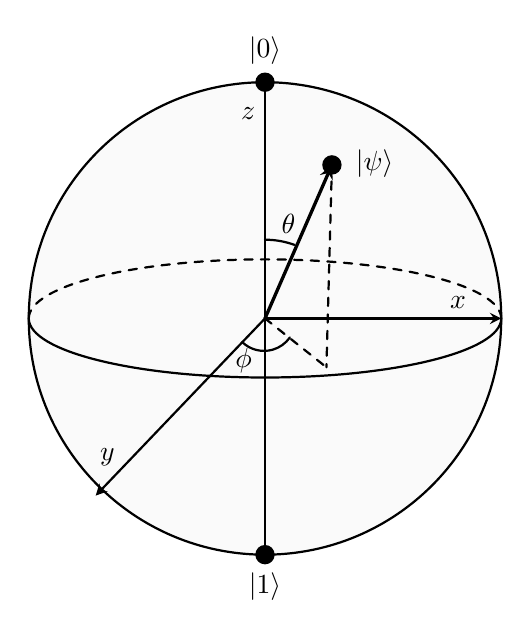
\begin{tikzpicture}[
			scale=1,
			line cap=round,
			line join=round,
			>=stealth
			]
			
			% Sphere
			\def\R{3}
			\draw[thick, fill=gray!4] (0,0) circle (\R);
			
			% Equator: hidden rear half and visible front half
			\draw[thick]
			(-\R,0) arc[start angle=180,end angle=360,
			x radius=\R,y radius=0.75];
			
			\draw[thick, dashed]
			(\R,0) arc[start angle=0,end angle=180,
			x radius=\R,y radius=0.75];
			
			% Coordinate axes
			\draw[thick] (0,0) -- (0,3);
			\draw[thick] (0,0) -- (0,-3);
			
			\draw[thick,->] (0,0) -- (-2.15,-2.25);
			\node[above] at (-2,-2) {$y$};
			\draw[thick,->]    (0,0) -- (3,0);
			\node[above] at (2.45,0) {$x$};
			\node[left] at (0,2.6) {$z$};
			
			% Bloch vector endpoint and its projection
			\coordinate (P) at (0.85,1.95);
			\coordinate (Q) at (0.78,-0.62);
			
			\draw[very thick,->] (0,0) -- (P);
			\fill (P) circle (3.5pt);
			
			% Dashed projection onto the equatorial plane
			\draw[thick,dashed] (P) -- (Q);
			\draw[thick,dashed] (0,0) -- (Q);
			
			% Polar angle theta
			\draw[thick]
			(0,1)
			arc[start angle=90,end angle=70,radius=1.1];
			
			\node at (0.3,1.2) {$\theta$};
			
			% Azimuthal angle phi
			\draw[thick]
			(-0.29,-0.3)
			arc[start angle=226,end angle=325,
			radius=0.4];
			
			\node at (-0.27,-0.53) {$\phi$};
			
			% Basis-state labels
			\fill (0,3) circle (3.5pt);
			\fill (0,-3) circle (3.5pt);
			
			\node[above] at (0,3.1) {$\ket{0}$};
			\node[below] at (0,-3.1) {$\ket{1}$};
			
			% State label
			\node[right] at ($(P)+(0.18,0.02)$) {$\ket{\psi}$};
			
		\end{tikzpicture}
	\end{center}
	The Bloch sphere is useful because it turns a two-level quantum state into geometry: measurement probabilities become projections, unitary evolution becomes rotation, and mixedness becomes distance from the center.
	\subsubsection{Visualizing a state as a point on the sphere}
	Choose \(|0\rangle=|\uparrow\rangle\) and \(|1\rangle=|\downarrow\rangle\). Any normalized pure qubit state, after removing an overall phase, can be written as
	\[
	|\psi\rangle=\cos\left(\tfrac{\theta}{2}\right)|0\rangle
	+e^{i\phi}\sin\left(\tfrac{\theta}{2}\right)|1\rangle
	\]Its Bloch vector is
	\[
	{\mathbf r=(\sin\theta\cos\phi,\;\sin\theta\sin\phi,\;\cos\theta).}
	\]
	which is the unit radial vector in spherical coordinates. Here \(\theta\) is the polar angle measured from \(+z\), and \(\phi\) is the azimuthal angle. \\ \\
	The half-angle in the ket makes it so that
	\begin{enumerate}[label=(\roman*)]
		\item \(|0\rangle\) and \(|1\rangle\) are the north and south poles
		\item \((|0\rangle\pm|1\rangle)/\sqrt2\) point along \(\pm x\) (often also notated $\ket{\rightarrow}$ and $\ket{\leftarrow}$ or $\ket{+}$ and $\ket{-}$)
		\item \((|0\rangle\pm i|1\rangle)/\sqrt2\) point along \(\pm y\)
		\item The Pauli expectations are equal to the cooresponding coordinate of the Bloch vector i.e. the projection onto the $x,y,z$ axes
		\begin{align*}
			\langle \hat{X}\rangle=\sin\theta\cos\phi\qquad,\qquad\langle \hat{Y}\rangle = \sin\theta\sin\phi\qquad,\qquad\langle \hat{Z}\rangle=\cos\theta
		\end{align*}
	\end{enumerate}
	Orthogonal kets correspond to antipodal points on the sphere, not perpendicular Bloch vectors. Multiplying a ket by an overall phase leaves its point unchanged while changing the relative phase moves it. \\ \\
	Other useful facts:
	\begin{enumerate}[label=(\roman*)]
		\item $\theta$ controls the measurement probabilies in the $z$-basis i.e.
		\begin{align*}
			P(Z=+1)=\cos^2(\theta/2)\qquad,\qquad P(Z=-1)=\sin^2(\theta/2)
		\end{align*}
	\end{enumerate}
	
	\section{Composite Quantum Systems}
	\subsection{Tensors}
	\begin{definition}
		Give a vector space $V$ of dimension $m$ and a vector space $W$ of dimension $n$, their \textit{\textbf{tensor product space}} is the vector space
		\begin{align*}
			V\otimes W \equiv \operatorname{span}\{\ket{v}\otimes\ket{w} \, \mid \, \ket{v}\in V, \ket{w}\in W\}
		\end{align*}
		of dimension $mn$. An element $\ket{\psi}$ of this vector space is called a \textit{\textbf{tensor}} and takes the form
		\begin{align*}
			\ket{\psi} = \sum_{i} a_i (\ket{v_i}\otimes\ket{w_i})
		\end{align*}
		The tensor product is \textit{\textbf{bilinear}} e.g.
		\[
		\ket{\psi} = \sum_i
		a_i\bigl(|v_i\rangle\otimes|w_i\rangle\bigr)
		=
		\sum_i
		\bigl(a_i|v_i\rangle\bigr)\otimes|w_i\rangle
		=
		\sum_i
		|v_i\rangle\otimes\bigl(a_i|w_i\rangle\bigr).
		\]
		The inner product on the tensor product space is defined
		\begin{align*}
			\bigl(\langle v|\otimes\langle w|\bigr)
			\bigl(|v'\rangle\otimes|w'\rangle\bigr)
			=\langle v|v'\rangle\,\langle w|w'\rangle
		\end{align*}
		Since the inner product is conjugate-linear in the first argument and linear in the second, if
		\[
		|\Psi\rangle=\sum_i a_i|v_i\rangle\otimes|w_i\rangle\qquad,
		\qquad
		|\Phi\rangle=\sum_j b_j|v'_j\rangle\otimes|w'_j\rangle
		\]
		then
		\[
		{
			\langle\Psi|\Phi\rangle
			=\sum_{i,j}a_i^*b_j
			\langle v_i|v'_j\rangle
			\langle w_i|w'_j\rangle.
		}
		\]
		For linear operators $\hat{A}$ on $V$ and $\hat{B}$ on $W$, we can construct a linear operator in the tensor product space
		\begin{align*}
			(\hat{A}\otimes\hat{B})(\ket{v}\otimes\ket{w}) = \hat{A}\ket{v}\otimes \hat{B}\ket{w}
		\end{align*}
	\end{definition}
	\begin{todo}
		Add explicit examples with matrices for clarity
	\end{todo}
	
	\subsection{Generalized Measurements}
	One way we can glean information about a system is to let it interact with another system that we can measure (called the ancilla). Consider two Hilbert spaces $\mathbb{V}_s$ (measured system) and $\mathbb{V}_a$ (ancilla system) and a state $\ket{\Psi}$ in their tensor product space
	\begin{align*}
		\ket{\Psi} \equiv \ket{\psi}_s \otimes \ket{\phi}_a
	\end{align*}
	evolving unitarily under a Hamiltonian $\hat{H}$ for time $t$. Suppose we perform a projective measurement on $\mathbb{V}_a$ associated with the linear operator $\mathds{1}\otimes \hat{P}_a$, where $\hat{P}_a$ has the spectral decomposition
	\begin{align*}
		\hat{P}_a = \sum_q \lambda_q \ket{q}\bra{q}
	\end{align*}
	and $\{\ket{q}\}$ forms a complete orthonormal basis for $\mathbb{V}_a$. Immediately before the measurement, the joint state is
	\begin{align*}
		\ket{\Psi'} = \hat{U}(\ket{\psi}_s \otimes \ket{\psi}_a)
	\end{align*}
	where $\hat{U}=e^{-i\hat{H}t/\hbar}$. After such a measurement with measurement outcome $\lambda_q$, the state collapses into a new (unnormalized) state $\hat{M}_q(\ket{\psi}_s\otimes \ket{\phi}_a)$
	where
	\begin{align*}
		\hat{M}_q \equiv {}_a\langle q | \hat{U} | \phi\rangle_a \in \mathbb{L}_{\mathbb{V}_s}
	\end{align*}
	is a linear operator on $\mathbb{V}_s$. In other words, $\hat{M}_q$ describes the effect on the first system associated with obtaining a measurement outcome $\lambda_q$ from the ancilla system. More explicitly,
	\begin{align*}
		\hat{M}_q|\psi\rangle_s
		=
		\bigl(\mathds{1}_s\otimes{}_a\langle q|\bigr)
		\hat U
		\bigl(|\psi\rangle_s\otimes|\phi\rangle_a\bigr)
	\end{align*}
	Reading from right to left, this means that we can obtain $\hat{M}_q\ket{\psi}_s$ by
	\begin{enumerate}
		\item Applying the joint evolution operator $\hat{U}$ to the initial joint state
		\begin{align*}
			\hat{U}(\ket{\psi}_s\otimes \ket{\phi}_a) = \sum_{i,j} c_{ij}(\ket{i}_s\otimes \ket{j}_a)
		\end{align*}
		\item Taking the inner product
		\[
		\begin{aligned}
			\bigg\langle\bigl(\mathds{1}_s\otimes{}_a\langle q|\bigr)\,\bigg\lvert\,
			\sum_{i,j}c_{ij}\bigl(|i\rangle_s\otimes|j\rangle_a\bigr)\bigg\rangle
			&=\sum_{i,j}c_{ij}|i\rangle_s
			\underbrace{{}_a\langle q|j\rangle_a}_{\delta_{qj}}
			&=\sum_{i,j}c_{ij}\delta_{qj}|i\rangle_s
				=\sum_i c_{iq}|i\rangle_s
		\end{aligned}
		\]
	\end{enumerate}
	Since
	\[
	\begin{aligned}
		\hat P_q|\Psi'\rangle
		&=
		\sum_j
		\bigl(\hat{M}_j|\psi\rangle_s\bigr)
		\otimes
		\bigl(|q\rangle_a\,{}_a\langle q|j\rangle_a\bigr)\\
		&=
		\sum_j
		\delta_{qj}\bigl(\hat{M}_j|\psi\rangle_s\bigr)\otimes|q\rangle_a\\
		&=
		{\hat{M}_q\bigl(|\psi\rangle_s\otimes|q\rangle_a}\bigr)
	\end{aligned}
	\]
	by the Born rule, the probability that a measurement on $\mathbb{V}_a$ produces $q$ is
	\begin{align*}
		\prob(q)  = \braket{\Psi' | \hat{P}_q | \Psi'} = {}_s\langle\psi | \hat{M}_q^\dagger \hat{M}_q | \psi\rangle_s
	\end{align*}
	thus the $\hat{M}_q$'s satisfy the completeness relation $\sum_{q} = \hat{M}_a^\dagger \hat{M}_q=\mathds{1}_s$. Alternatively, we can also write
	\begin{align*}
		\prob(q) = \operatorname{tr}(\hat{M}_q\ket{\psi}_s\bra{\psi}_s \hat{M}_q^\dagger
	\end{align*}
	\begin{example}
		\begin{todo}
			Add examples for clarity
		\end{todo}
	\end{example}
	
	\section{Density Matrices, Mixed States, Entanglement}
	\begin{definition}
		Suppose we have a system that is described by normalized (but not necessarily orthogonal) states $\ket{\psi_i}$ with probability $p_i$. This system can then be described by a \textit{\textbf{density matrix}}
		\begin{align*}
			\hat{\rho} = \sum_{i} p_i \ket{\psi_i}\bra{\psi_i}
		\end{align*}
		Then, the expactation value of any operator $\hat{A}$ is
		\begin{align*}
			\avg{\hat{A}} = \sum_{i} p_i \braket{\psi_i | \hat{A} | \psi_i} = \operatorname{tr}(\hat{\rho}\hat{A})
		\end{align*}
		If the system is described by a specific state $\psi$, we call it a \textit{\textbf{pure state}} $\iff$
		\begin{align*}
			\hat{\rho} = \ket{\psi}\bra{\psi} \quad,\quad \hat{\rho}^2 = \hat{\rho}
		\end{align*}
		is simply the projection operator. A state that is not pure is called a \textit{\textbf{mixed state}}.
	\end{definition}
	\subsection{Properties of the Density Matrix}
	The density matrix has the following properties:
	\begin{enumerate}[label=(\roman*)]
		\item It is self-adjoint: $\hat{\rho} = \hat{\rho}^\dagger$.
		
		\item It has unit trace: $\operatorname{tr}(\hat{\rho}) = 1$.
		\begin{equation*}
			\begin{aligned}
				\operatorname{tr}(\hat{\rho})
				&= \sum_n \bra{n}\hat{\rho}\ket{n}
				= \sum_n \sum_i
				p_i \braket{n}{\psi_i}\braket{\psi_i}{n} \\
				&= \sum_i p_i \sum_n
				\braket{\psi_i}{n}\braket{n}{\psi_i}
				= \sum_i p_i \braket{\psi_i}{\psi_i}
				= 1.
			\end{aligned}
		\end{equation*}
		
		Here, in an intermediate step, we needed to use the
		decomposition of unity
		$\sum_n \ket{n}\bra{n} = \mathds{1}$ and, in the final
		step, we used the fact that our states $\ket{\psi_i}$
		are normalised. We see that the fact the density matrix
		has unit trace is equivalent to the normalisation of
		a probability distribution, $\sum_i p_i = 1$.
		
		\item It is non-negative i.e. $\hat{\rho} \geq 0$:
		$\bra{\phi}\hat{\rho}\ket{\phi} \geq 0$
		for all $\ket{\phi} \in \mathcal{H}$.
		This is equivalent to the requirement
		that $p_i \geq 0$.
	\end{enumerate}
	
	Any operator $\hat{\rho}$ which satisfies these three
	properties can be viewed as a density matrix for a quantum
	system. To see this, suppose $\{\ket{\phi_n}\}$ are eigenvectors of $\hat{\rho}$ with eigenvalues $\{p_n\}$. Then
	\begin{equation*}
		\hat{\rho}\ket{\phi_n} = p_n\ket{\phi_n}
	\end{equation*}
	Because $\hat{\rho} = \hat{\rho}^\dagger$, we know that
	$p_n \in \mathbb{R}$. Properties (ii) and (iii) above $\implies \sum_n p_n = 1$ and $p_n \geq 0\implies$ we can interpret$\{p_n\}$ as a probability
	distribution and write $\hat{\rho}$ as
	\begin{equation*}
		\hat{\rho} = \sum_n p_n\ket{\phi_n}\bra{\phi_n}
	\end{equation*}
	\begin{todo}
		Add how it relates back to the Bloch sphere (pages 1067-1070 in Tong)
	\end{todo}
	
	\subsection{Entanglement}
	\begin{definition}
		A Hilbert space $\mathcal{H}$ has a \textit{\textbf{bipartite decomposition}} if it can be expressed as the tensor product space of two Hilbert spaces $\mathcal{H} = \mathcal{H}_A \otimes \mathcal{H}_B$.
	\end{definition}
	If $\{\ket{i}_A\}$ and $\{\ket{j}_B\}$ are orthonormal bases for $\mathcal{H}_A$ and $\mathcal{H}_B$, then a general composite state $\ket{\Psi}\in\mathcal{H}$ has the form
	\begin{align*}
		\ket{\Psi} = \sum_{i,j} c_{ij}(\ket{i}_A \otimes \ket{j}_B)
	\end{align*}
	All measurements on only $\mathcal{H}_A$ correspond to operators of the form $\hat{O} = \hat{A}\otimes \mathds{1}$. If $\hat{\rho}_{AB}$ is the density matrix for the full system, then the expectation value of
	\begin{align*}
		\avg{\hat{A}} = \operatorname{tr}_A\operatorname{tr}_B\left((\hat{A}\otimes\mathds{1})\hat{\rho}_{AB}\right) = \operatorname{tr}_A(\hat{A}\hat{\rho}_A)
	\end{align*}
	where $\hat{\rho}_A = \operatorname{tr}_B(\hat{\rho}_{AB})$ is the \textit{\textbf{reduced density matrix}} which is obtained by taking the partial trace over $\mathcal{H}_B$.
	
	\begin{example}
		Consider two matrices $A^{m\x m}$ and $B^{n\x n}$ (which could represent linear operators).
		
		Then
		\begin{align*}
			A\otimes B =
			\begin{pmatrix}
				a_{11} B & \cdots & a_{1m} B \\
				\vdots & \ddots & \vdots \\
				a_{m1} B & \cdots & a_{mm} B
			\end{pmatrix}
		\end{align*}
		and $\operatorname{tr}(A\otimes B) = a_{11}\operatorname{tr}(B) + \cdots + a_{mm}\operatorname{tr}(B)=\operatorname{tr}(A)\operatorname{tr}(B)$ is a scalar, but the partial traces
		\begin{align*}
			\operatorname{tr}_B(A\otimes B) = 
			\begin{pmatrix}
				a_{11} \operatorname{tr}(B) & \cdots & a_{1m} \operatorname{tr}(B) \\
				\vdots & \ddots & \vdots \\
				a_{m1} \operatorname{tr}(B) & \cdots & a_{mm} \operatorname{tr}(B)
			\end{pmatrix} = \operatorname{tr}(B) A
		\end{align*}
		\begin{align*}
			\operatorname{tr}_A(A\otimes B) =
			\begin{pmatrix}
				b_{11} \operatorname{tr}(A) & \cdots & b_{1n} \operatorname{tr}(A) \\
				\vdots & \ddots & \vdots \\
				b_{n1} \operatorname{tr}(A) & \cdots & b_{nn} \operatorname{tr}(A)
			\end{pmatrix}
			=\operatorname{tr}(A) B
		\end{align*}
		are matrices.
	\end{example}
	
	\begin{todo}
		Add Schmidt decomposition
	\end{todo}
%	\section{Appendix, Proofs of Theorems and Lemmas}
%	\begin{theorem}
%		\textit{\textbf{Spectral Decomposition Theorem}}
%		A linear operator \(\hat O\) on \(V\) is diagonal with respect to some orthonormal basis of \(V\) if and only if \(\hat O\) is normal, i.e.
%		$\hat O^\dagger\hat O=\hat O\hat O^\dagger$
%	\end{theorem}
%	\begin{proof}
%		Being diagonal in an orthonormal basis means that
%		\[
%		\hat O=\sum_i O_i|i\rangle\langle i|,
%		\tag{1.53}
%		\]
%		where the \(|i\rangle\) form a complete orthonormal basis and
%		\[
%		\hat O|i\rangle=O_i|i\rangle.
%		\]
%		Proof: an orthonormal eigenbasis implies normality.
%		Suppose \(\hat O\) has the form (1.53). Taking its adjoint gives
%		\[
%		\hat O^\dagger=\sum_i O_i^*|i\rangle\langle i|.
%		\]
%		Using \(\langle i|j\rangle=\delta_{ij}\),
%		\[
%		\begin{aligned}
%			\hat O^\dagger\hat O
%			&=\sum_{i,j}O_i^*O_j
%			|i\rangle\langle i|j\rangle\langle j|\\
%			&=\sum_i|O_i|^2|i\rangle\langle i|.
%		\end{aligned}
%		\]
%		Similarly,
%		\[
%		\hat O\hat O^\dagger
%		=\sum_i|O_i|^2|i\rangle\langle i|.
%		\]
%		Therefore \(\hat O^\dagger\hat O=\hat O\hat O^\dagger\).
%		Proof: normality implies an orthonormal eigenbasis.
%		We first establish a useful fact. If \(\hat O\) is normal and
%		\[
%		\hat O|v\rangle=\lambda|v\rangle,
%		\]
%		then
%		\[
%		\hat O^\dagger|v\rangle=\lambda^*|v\rangle.
%		\]
%		To prove this, define
%		\[
%		\hat A=\hat O-\lambda\mathds{1}.
%		\]
%		Normality of \(\hat O\) implies normality of \(\hat A\), because
%		\[
%		\hat A^\dagger\hat A-\hat A\hat A^\dagger
%		=\hat O^\dagger\hat O-\hat O\hat O^\dagger=0.
%		\]
%		Consequently,
%		\[
%		\begin{aligned}
%			\|\hat A^\dagger|v\rangle\|^2
%			&=\langle v|\hat A\hat A^\dagger|v\rangle\\
%			&=\langle v|\hat A^\dagger\hat A|v\rangle\\
%			&=\|\hat A|v\rangle\|^2=0.
%		\end{aligned}
%		\]
%		Thus \(\hat A^\dagger|v\rangle=0\), proving the fact.
%		We now use induction on \(n=\dim V\). The result is immediate for \(n=1\).
%		For \(n>1\), a complex matrix has at least one eigenvalue, so choose a normalized eigenvector \(|1\rangle\):
%		\[
%		\hat O|1\rangle=\lambda_1|1\rangle,
%		\qquad
%		\hat O^\dagger|1\rangle=\lambda_1^*|1\rangle.
%		\]
%		Consider its orthogonal complement
%		\[
%		W=\{|w\rangle\in V:\langle1|w\rangle=0\}.
%		\]
%		For any \(|w\rangle\in W\),
%		\[
%		\langle1|\hat O|w\rangle
%		=\lambda_1\langle1|w\rangle=0,
%		\]
%		where we used the adjoint of
%		\(\hat O^\dagger|1\rangle=\lambda_1^*|1\rangle\).
%		Likewise,
%		\[
%		\langle1|\hat O^\dagger|w\rangle
%		=\lambda_1^*\langle1|w\rangle=0.
%		\]
%		Therefore both \(\hat O\) and \(\hat O^\dagger\) map \(W\) into itself. Their restrictions to \(W\) still commute, so the restriction of \(\hat O\) is normal.
%		Since \(\dim W=n-1\), the induction hypothesis supplies an orthonormal eigenbasis
%		\[
%		|2\rangle,\ldots,|n\rangle
%		\]
%		for \(W\). Together with \(|1\rangle\), these form a complete orthonormal eigenbasis for \(V\). Hence
%		\[
%		\hat O=\sum_i\lambda_i|i\rangle\langle i|
%		\]
%	\end{proof}
%	\begin{theorem}
%		A normal matrix is Hermitian if and only if it has real eigenvalues
%	\end{theorem}
%	\begin{proof}
%		By Theorem 2.1, a normal operator has a spectral decomposition
%		\[
%		\hat O=\sum_i\lambda_i|i\rangle\langle i|,
%		\qquad
%		\hat O^\dagger=\sum_i\lambda_i^*|i\rangle\langle i|.
%		\]
%		If \(\hat O\) is Hermitian, then
%		\[
%		\lambda_i
%		=\langle i|\hat O|i\rangle
%		=\langle i|\hat O^\dagger|i\rangle
%		=\lambda_i^*,
%		\]
%		so every eigenvalue is real.
%		Conversely, if all \(\lambda_i\) are real, then
%		\[
%		\hat O^\dagger
%		=\sum_i\lambda_i^*|i\rangle\langle i|
%		=\sum_i\lambda_i|i\rangle\langle i|
%		=\hat O.
%		\]
%		Thus \(\hat O\) is Hermitian.
%	\end{proof}
%	\begin{theorem}
%		Eigenkets corresponding to different eigenvalues of a Hermitian matrix are orthogonal
%	\end{theorem}
%	\begin{proof}
%		Let \(\hat M=\hat M^\dagger\), and suppose
%		\[
%		\hat M|i\rangle=\lambda_i|i\rangle,
%		\qquad
%		\hat M|j\rangle=\lambda_j|j\rangle,
%		\qquad
%		\lambda_i\ne\lambda_j.
%		\]
%		A Hermitian operator is normal, so Theorem 2.2 tells us that its eigenvalues are real. Taking the adjoint of the first eigenvalue equation gives
%		\[
%		\langle i|\hat M=\lambda_i\langle i|.
%		\]
%		Now evaluate the same matrix element in two ways:
%		\[
%		\langle i|\hat M|j\rangle
%		=\lambda_j\langle i|j\rangle
%		\]
%		by acting to the right, while
%		\[
%		\langle i|\hat M|j\rangle
%		=\lambda_i\langle i|j\rangle
%		\]
%		by acting to the left. Subtracting,
%		\[
%		(\lambda_i-\lambda_j)\langle i|j\rangle=0.
%		\]
%		Since \(\lambda_i\ne\lambda_j\),
%		\[
%		{\langle i|j\rangle=0}
%		\]
%		For equal eigenvalues, this argument imposes no condition on the overlap. Vectors within a degenerate eigenspace need not initially be orthogonal, but an orthonormal basis can be chosen there.
%	\end{proof}
%	\begin{theorem}
%		A positive linear operator must be Hermitian. Here positive means
%		\[
%		\langle v|\hat O|v\rangle\geq0
%		\]
%		for every \(|v\rangle\in V\). In particular, every such expectation value is real. Hermiticity is not assumed in this definition.
%	\end{theorem}
%	\begin{proof}
%		Decompose \(\hat O\) into its Hermitian and anti-Hermitian parts:
%		\[
%		\hat O=\hat H+i\hat K,
%		\]
%		where
%		\[
%		\hat H=\frac{\hat O+\hat O^\dagger}{2},
%		\qquad
%		\hat K=\frac{\hat O-\hat O^\dagger}{2i}.
%		\]
%		Directly taking adjoints shows
%		\[
%		\hat H^\dagger=\hat H,
%		\qquad
%		\hat K^\dagger=\hat K.
%		\]
%		For every \(|v\rangle\),
%		\[
%		\langle v|\hat O|v\rangle
%		=
%		\langle v|\hat H|v\rangle
%		+i\langle v|\hat K|v\rangle.
%		\]
%		Both expectations on the right are real because \(\hat H,\hat K\) are Hermitian. Positivity requires the left side to be real, so its imaginary part vanishes:
%		\[
%		\langle v|\hat K|v\rangle=0
%		\quad\text{for every }|v\rangle.
%		\]
%		Since \(\hat K\) is Hermitian, it has a complete orthonormal eigenbasis. For any normalized eigenvector \(|i\rangle\),
%		\[
%		\hat K|i\rangle=k_i|i\rangle
%		\quad\Longrightarrow\quad
%		k_i=\langle i|\hat K|i\rangle=0.
%		\]
%		All eigenvalues vanish, hence \(\hat K=0\). Therefore
%		\[
%		\boxed{\hat O=\hat H=\hat O^\dagger.}
%		\]
%		In fact, this proof shows that real expectation values for every vector already imply Hermiticity. Nonnegativity further ensures that the eigenvalues are nonnegative.
%	\end{proof}
%	\begin{theorem}
%		\textbf{\textit{Simultaneous diagonalization theorem}}
%		Two Hermitian linear operators \(\hat A\) and \(\hat B\) can be diagonalized simultaneously if and only if
%		\[
%		\boxed{[\hat A,\hat B]=0.}
%		\]
%		In other words, there is a complete orthonormal basis of simultaneous eigenkets:
%		\[
%		\hat A|a,b\rangle=a|a,b\rangle,
%		\qquad
%		\hat B|a,b\rangle=b|a,b\rangle.
%		\tag{1.55}
%		\]
%		If several independent states have the same pair of eigenvalues, an additional label is needed.
%		Proof: simultaneous diagonalization implies commutation.
%		Using conventional basis indices, suppose
%		\[
%		\hat A|i\rangle=a_i|i\rangle,
%		\qquad
%		\hat B|i\rangle=b_i|i\rangle
%		\]
%		for every vector in a complete basis. Then
%		\[
%		\hat A\hat B|i\rangle
%		=a_ib_i|i\rangle
%		=\hat B\hat A|i\rangle.
%		\]
%		Thus
%		\[
%		[\hat A,\hat B]|i\rangle=0
%		\]
%		for every basis vector. By linearity, the commutator vanishes on every vector:
%		\[
%		[\hat A,\hat B]=0.
%		\]
%	\end{theorem}
%	\begin{proof}
%		Commutation implies simultaneous diagonalization.
%		Suppose \([\hat A,\hat B]=0\). Since \(\hat A\) is Hermitian, \(V\) decomposes into its mutually orthogonal eigenspaces.
%		Let \(V_a\) be the eigenspace with eigenvalue \(a\). For any \(|v\rangle\in V_a\),
%		\[
%		\hat A|v\rangle=a|v\rangle.
%		\]
%		Using commutation,
%		\[
%		\begin{aligned}
%			\hat A(\hat B|v\rangle)
%			&=\hat B\hat A|v\rangle\\
%			&=\hat B(a|v\rangle)\\
%			&=a(\hat B|v\rangle).
%		\end{aligned}
%		\]
%		Therefore \(\hat B|v\rangle\) also belongs to \(V_a\): \(\hat B\) preserves every eigenspace of \(\hat A\).
%		Restrict \(\hat B\) to one such eigenspace \(V_a\). This restriction is still Hermitian, so it has an orthonormal eigenbasis within \(V_a\). Every vector in that basis is:
%		- an eigenvector of \(\hat A\), because it belongs to \(V_a\);
%		- an eigenvector of \(\hat B\), by construction.
%		Perform this diagonalization separately in every eigenspace of \(\hat A\). Combining the resulting bases gives a complete orthonormal basis of simultaneous eigenvectors for \(V\). \(\square\)
%		The degenerate case is the important step: commutation does not guarantee that every arbitrarily chosen eigenbasis of \(\hat A\) already diagonalizes \(\hat B\). It guarantees that we can choose suitable vectors within each degenerate eigenspace.
%		The spectral-projector form at the bottom of the page
%		A Hermitian operator has an orthonormal eigenbasis in which
%		\[
%		\hat M=\sum_i\lambda_i|i\rangle\langle i|.
%		\tag{1.56}
%		\]
%		If \(m\) labels the distinct eigenvalues, group all basis vectors sharing each eigenvalue:
%		\[
%		\boxed{
%			\hat M=\sum_m m\hat P_m,
%			\qquad
%			\hat P_m=\sum_j\delta_{\lambda_j,m}|j\rangle\langle j|.
%		}
%		\]
%		The operator \(\hat P_m\) projects onto the entire eigenspace with eigenvalue \(m\). Indeed,
%		\[
%		\begin{aligned}
%			\sum_m m\hat P_m
%			&=\sum_m\sum_jm\,\delta_{\lambda_j,m}|j\rangle\langle j|\\
%			&=\sum_j\lambda_j|j\rangle\langle j|\\
%			&=\hat M.
%		\end{aligned}
%		\]
%		For each fixed \(j\), only the term \(m=\lambda_j\) survives. This form makes degeneracy explicit without requiring a particular basis inside each eigenspace.
%	\end{proof}
	
\end{document}